\documentclass[english]{scrartcl}
\usepackage[T1]{fontenc}
\usepackage[utf8]{inputenc}
\usepackage[scaled=.8]{beramono}
\usepackage{geometry}
\geometry{verbose,tmargin=3cm,bmargin=3cm,lmargin=3cm,rmargin=3cm}
\usepackage{microtype}
\usepackage[parfill]{parskip}
\usepackage{amsmath}
\usepackage{graphicx}
\usepackage{hyperref}
\usepackage{nameref}
\usepackage{float}
\usepackage{listings}
\usepackage{color}
\usepackage{fancyhdr}
\usepackage{blindtext}

\usepackage{subcaption}

\pagestyle{fancy}
\fancyhf{}
\rhead{Team 3}
\lhead{BUSII}
\cfoot{\thepage}

\newcommand*{\fullref}[1]{\hyperref[{#1}]{\autoref*{#1}~\nameref*{#1}}}

\definecolor{darkgray}{rgb}{0.66, 0.66, 0.66}
\definecolor{asparagus}{rgb}{0.53, 0.66, 0.42}

\lstdefinestyle{s}{
  commentstyle=\color{darkgray},
  keywordstyle=\bfseries,
  morekeywords={},
  stringstyle=\color{asparagus},
  basicstyle=\ttfamily\footnotesize,
  breakatwhitespace=false,
  keepspaces=true,
  numbersep=5pt,
  showspaces=false,
  showstringspaces=false,
}

\lstset{style=s}

\begin{document}

\title{BUSII}

\author{Team 3}

\maketitle
\tableofcontents

\section{Visual Analysis of New Data}

We were given a different, much smaller data set which includes both line numbers
for indicating the progress in the driver program and rotational axes.

\subsection{Line numbers}

The line numbers are fairly straight forward: they are an integer, taking some positive value or -2.
We assume -2 means that the program is stopped. This is very well-behaved data which clearly shows
what is going on, which is a breath of fresh air. Figures~\ref{fig:linenumbers-real}~and~\ref{fig:linenumbers-sim} shows the line numbers
for both processes visualized as step functions over time.

\begin{figure}
    \begin{subfigure}[t]{0.5\textwidth}
        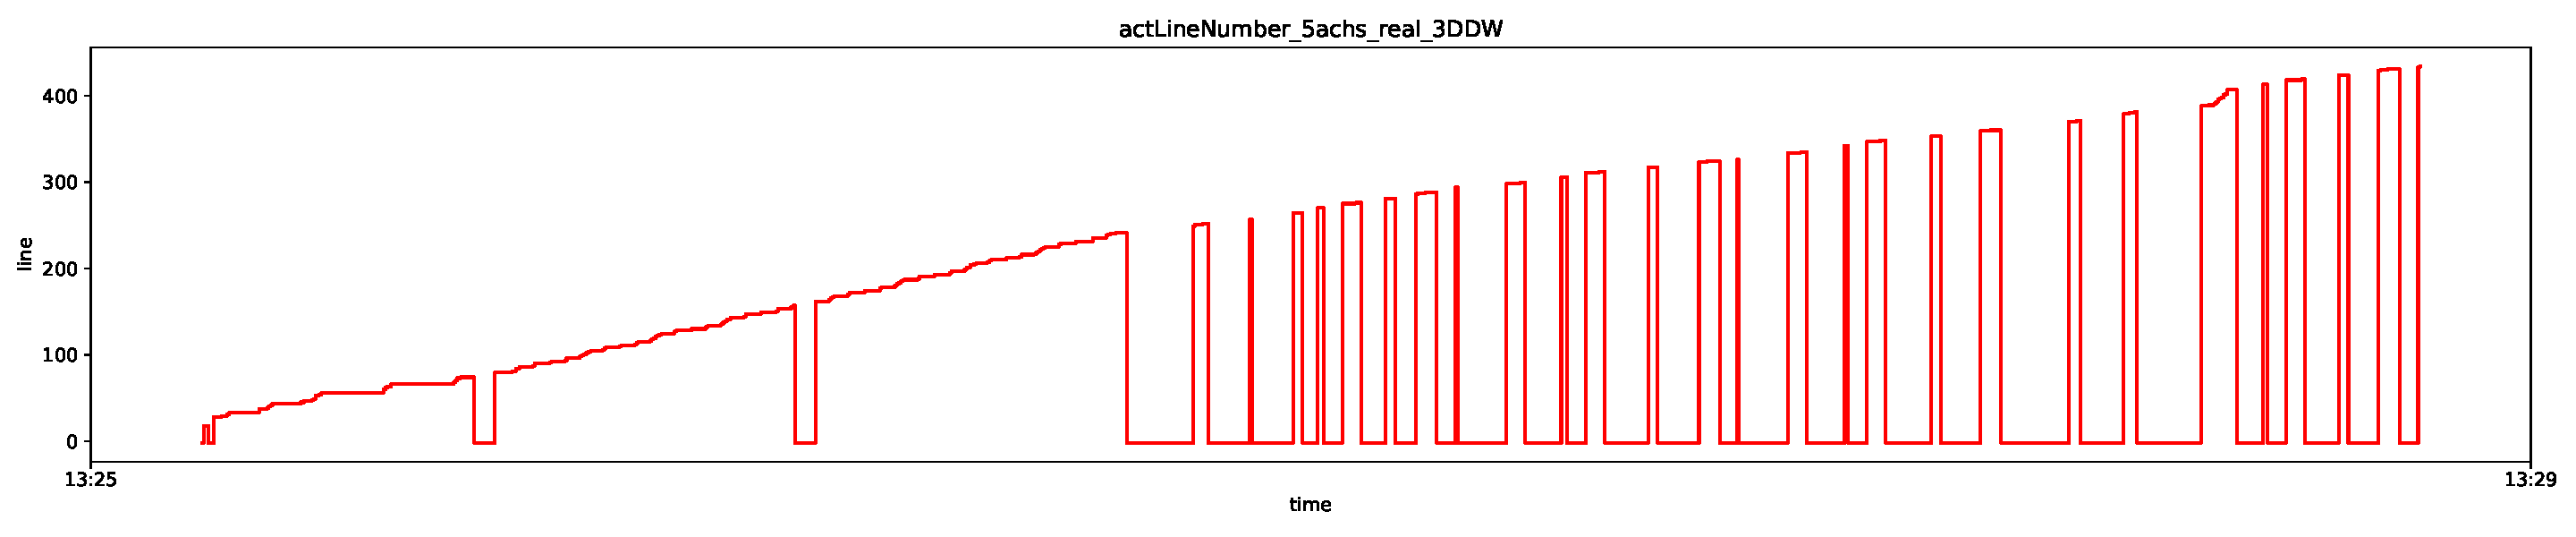
\includegraphics[width=\textwidth]{actLineNumber_real.pdf}
        \caption{Line numbers for the ``real'' process}
        \label{fig:linenumbers-real}
    \end{subfigure}%
    ~
    \begin{subfigure}[t]{0.5\textwidth}
        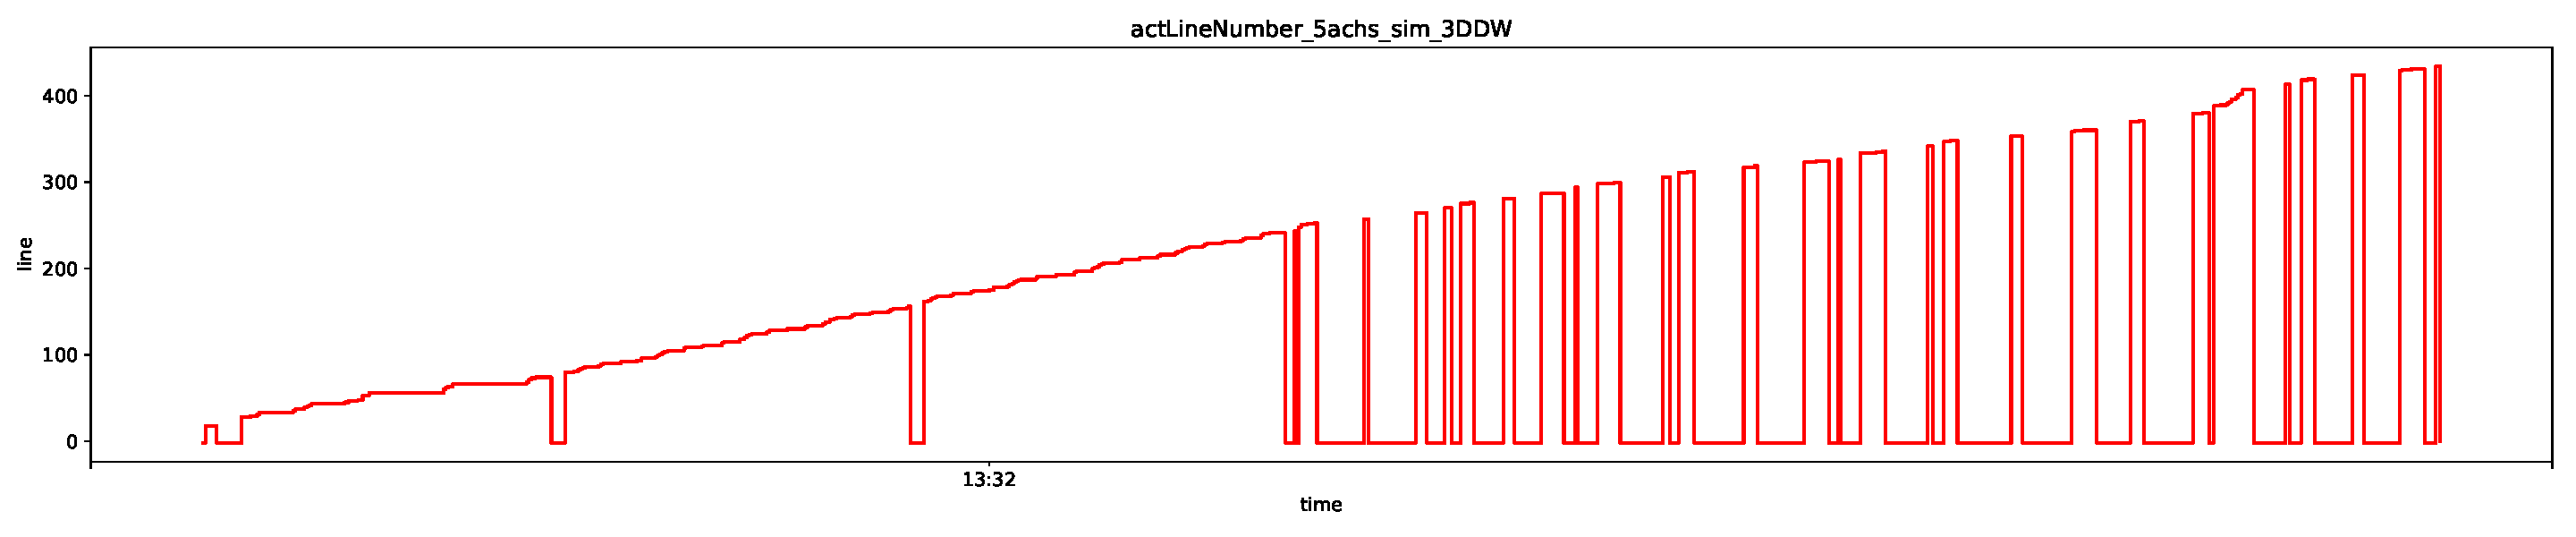
\includegraphics[width=\textwidth]{actLineNumber_sim.pdf}
        \caption{Line numbers for the ``sim'' process}
        \label{fig:linenumbers-sim}
    \end{subfigure}%
    \\
    \begin{subfigure}[t]{0.5\textwidth}
        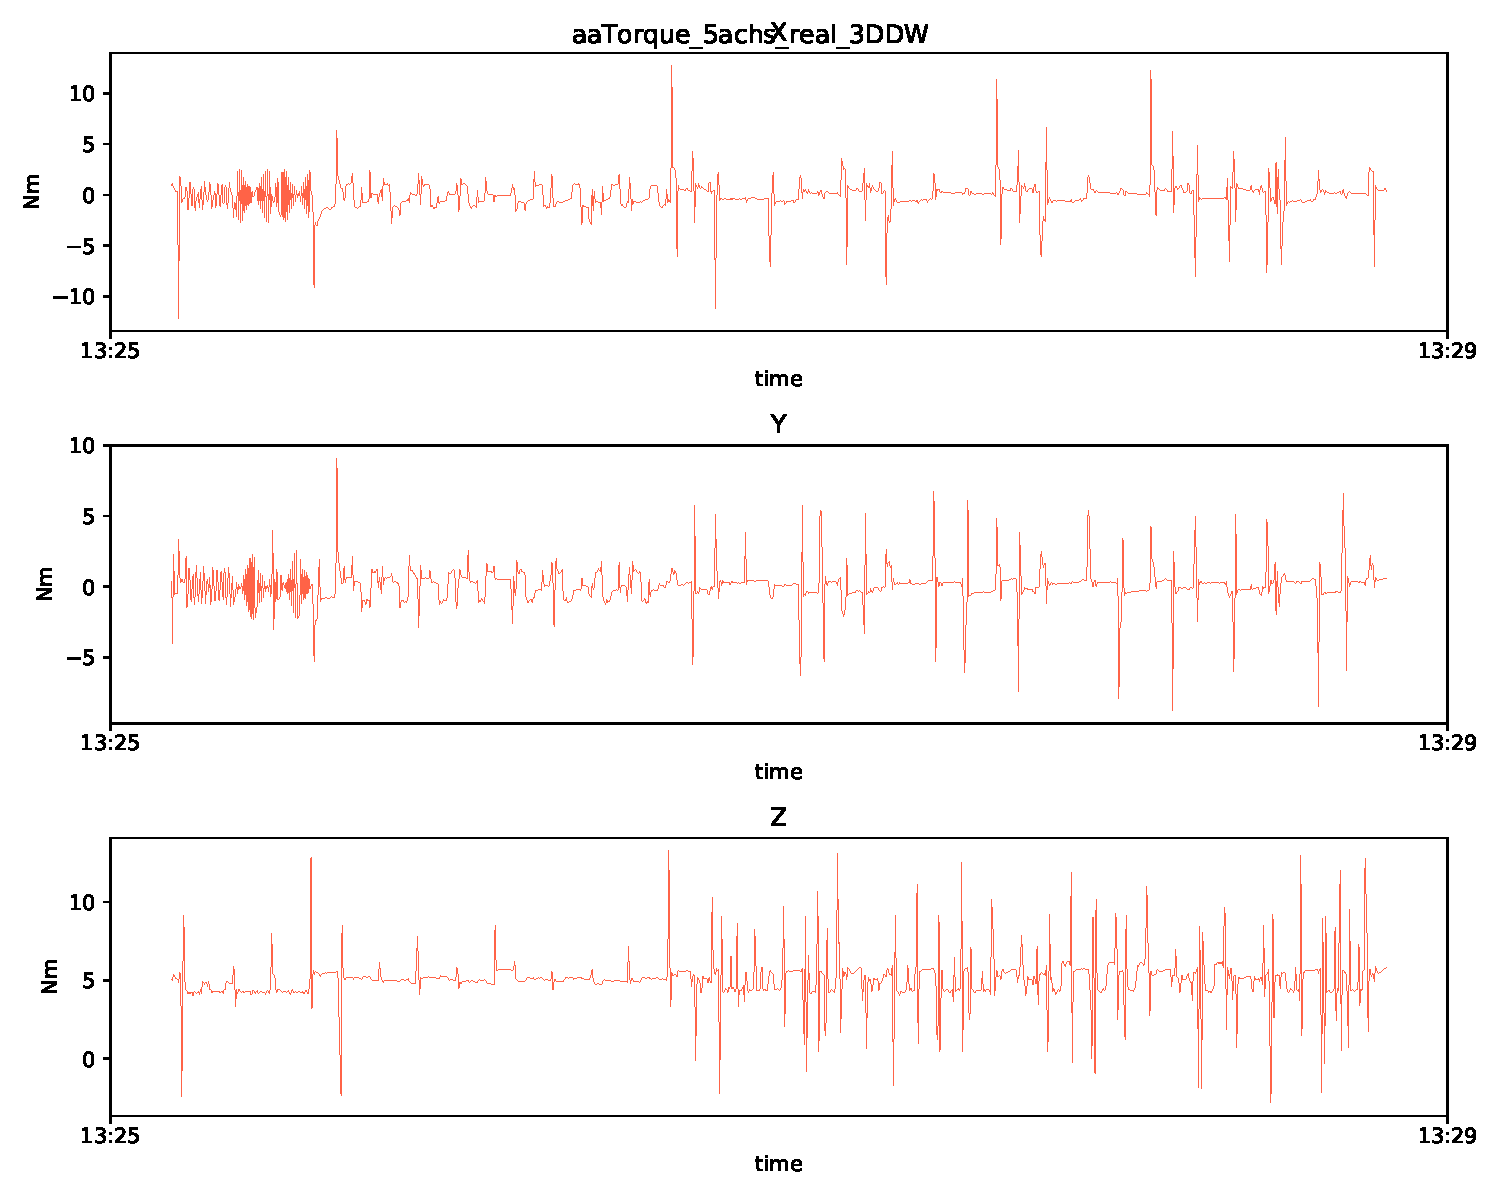
\includegraphics[width=\textwidth]{real_torque.pdf}
        \caption{Torque for the ``real'' process}
    \end{subfigure}%
    ~
    \begin{subfigure}[t]{0.5\textwidth}
        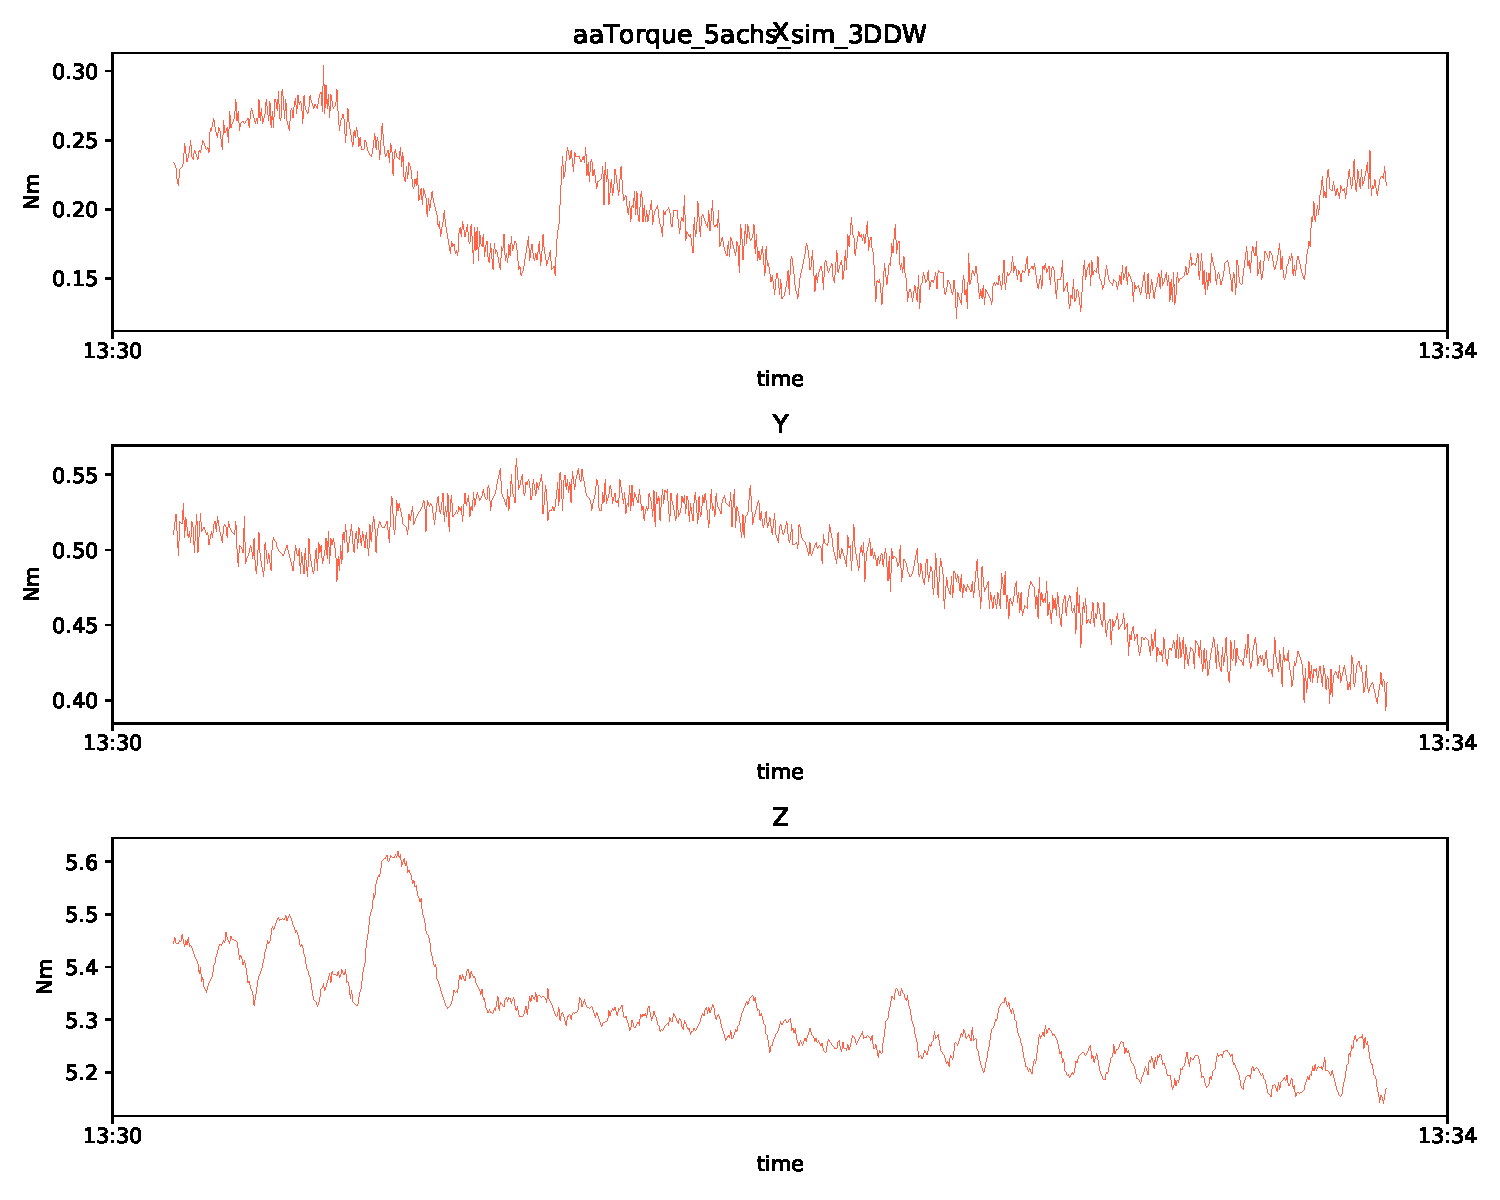
\includegraphics[width=\textwidth]{sim_torque.pdf}
        \caption{Torque for the ``sim'' process}
    \end{subfigure}%
    \\
    \begin{subfigure}[t]{0.5\textwidth}
        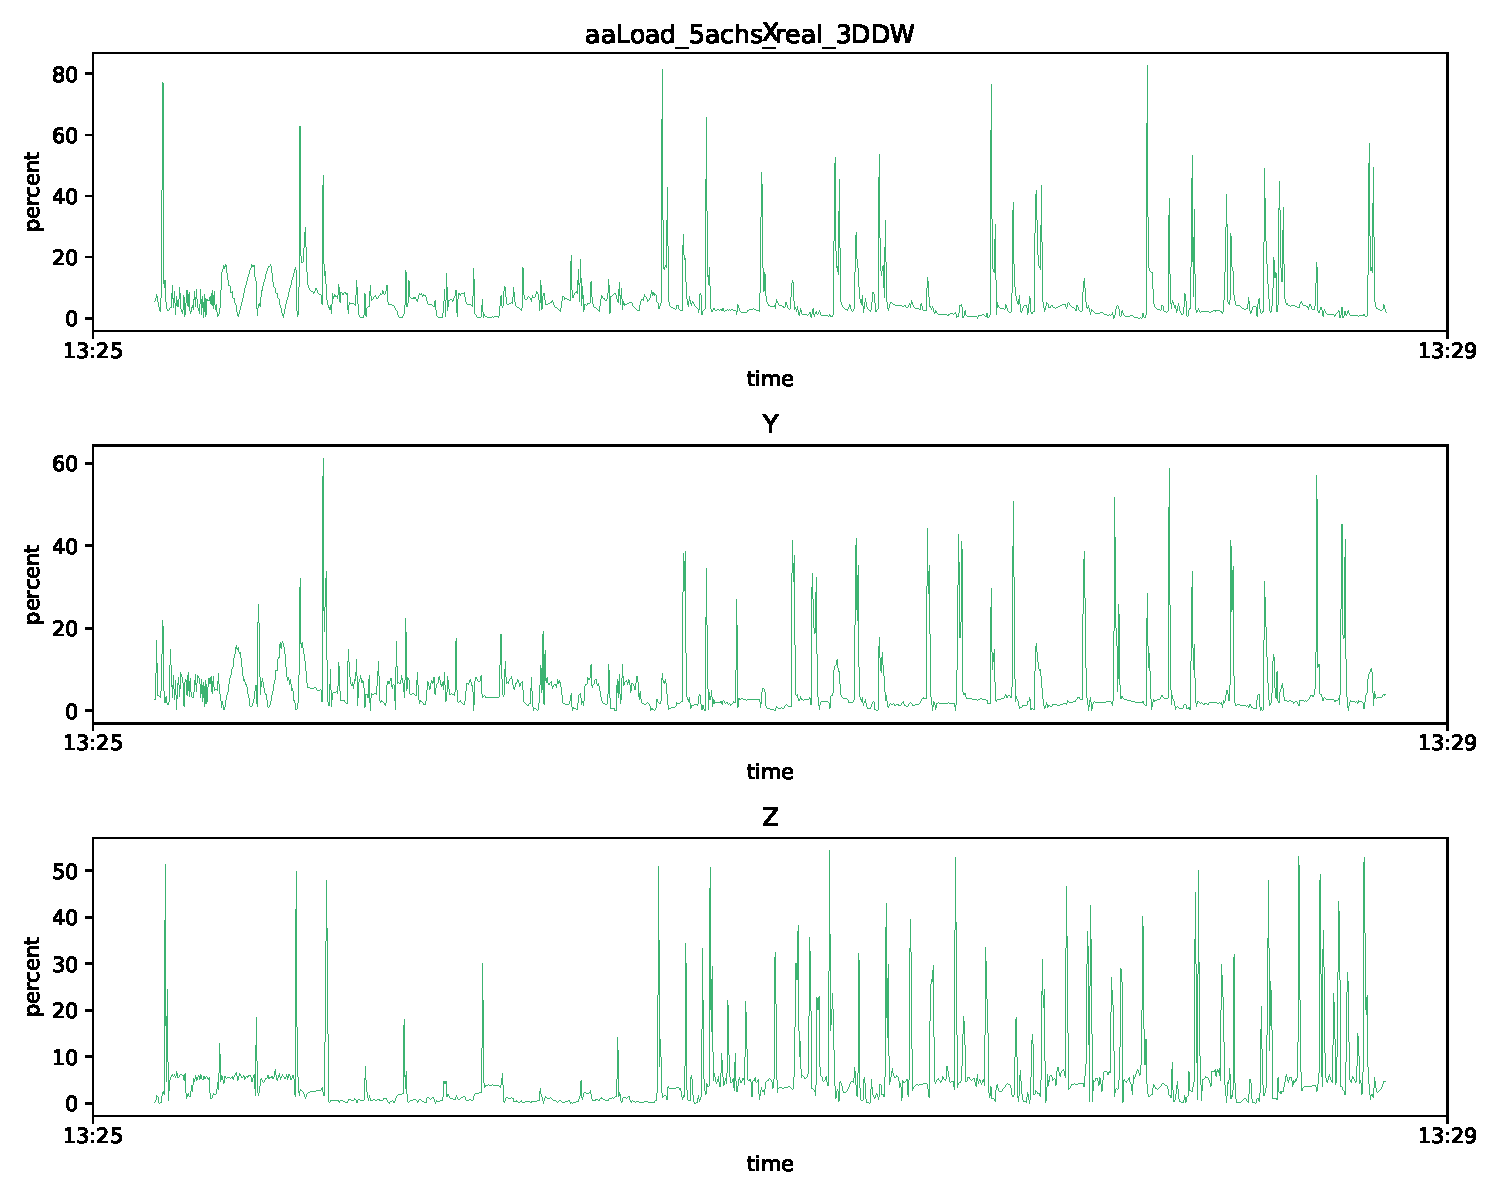
\includegraphics[width=\textwidth]{real_load.pdf}
        \caption{Drive load for the ``real'' process}
    \end{subfigure}%
    ~
    \begin{subfigure}[t]{0.5\textwidth}
        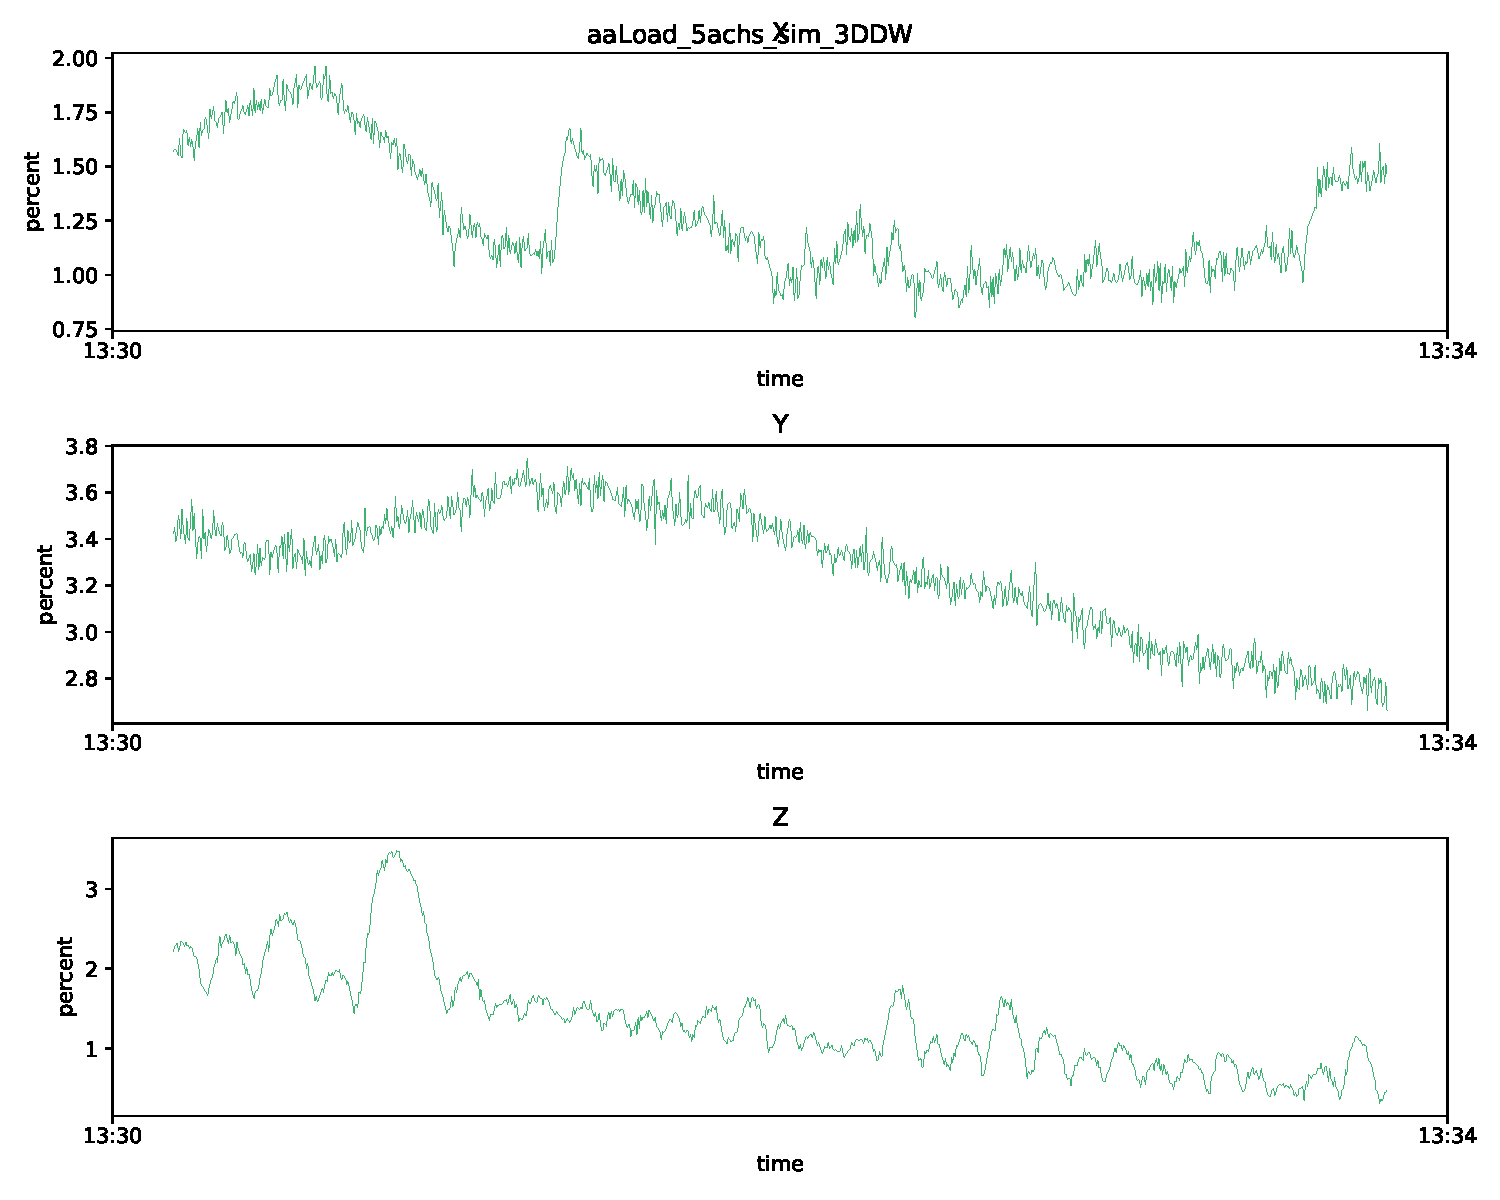
\includegraphics[width=\textwidth]{sim_load.pdf}
        \caption{Drive load for the ``sim'' process}
    \end{subfigure}%

    \caption{Plots illustrating differences between the two processes}
    \label{fig:diff}
\end{figure}

Both processes appear to behave quite similarly. They can roughly be divided into three first
segments which end with a stop, and then the latter half contains many stops. We can only assume
that the work done later is either more difficult, requiring stops to recalibrate or check things,
or that it is a simple finishing step which requires human checks whether it is finished.

The question however is as always: but what do they \emph{do}?! To this end,
take a look at the other plots of Figure~\ref{fig:diff}. There we can see that the
two processes look very different. The \emph{sim} process looks almost pretty
with its wavy curves---but most important of all, look at the magnitudes of the
values. They are \emph{much} lower than for the \emph{real} process---it is
thus pretty clear that \emph{sim} probably stands for ``simulated'', and the
machine did not actually mill, but only went through the motions, possibly
performing the probing routine. We've left out the axis speeds because the two
plots are quite similar.

\subsection{Rotation of coordinates}

The other interesting thing about this data set is the inclusion of the $B$ and $C$ axes. They
are both rotational axes, with $B$ rotating around the $Y$ axis, and $C$ around the $Z$ axis.

At first we thought this would be easy---we will construct a rotation matrix $R_{BC}$ and transform the vector
$v = \begin{pmatrix} x & y & z \end{pmatrix}^T$ by doing $v' = R_{BC} \cdot v$ and there they are, the actual coordinates.
However, this assumes that the rotation is occuring around the origin, which does not seem to be a valid assumption.

We assume that this is invalid because it does not work. Although some structure is revealed, it looks weird
and incomplete, and it seems like there still are two parts that should be connected, but are not.

We took to the internet and found out that what we are interested is \emph{CNC kinematics}. We found this link
\url{http://linuxcnc.org/docs/devel/html/motion/5-axis-kinematics.html}, which has some illustrations that might
be helpful, but at present are mostly overwhelming.

The possible explanations for this are (1) it is more complicated than we first assumed, (2) we did something wrong, or
(3) and most likely, both. However, the most pressing issue right now seems: where is the pivot. Which point in the
$(x, y, z)$ space are the $B$ and $C$ axes rotating around? It does not seem to be the origin, and figuring this out
from the data seems not very possible.

One issue that must be fixed is that the order of rotation needs to be considered---matrix multiplication is not
commutative and thus it makes a difference whether we rotate around $B$ and then around $C$ (resulting in the
rotation matrix $R_{CB} = R_CR_B$). Currently we are assuming that this is done in the reverse order for no particular
reason.

Figure~\ref{fig:rot} shows our failed attempt at reconstructing the object using rotation.

\begin{figure}
    \begin{subfigure}[t]{0.5\textwidth}
        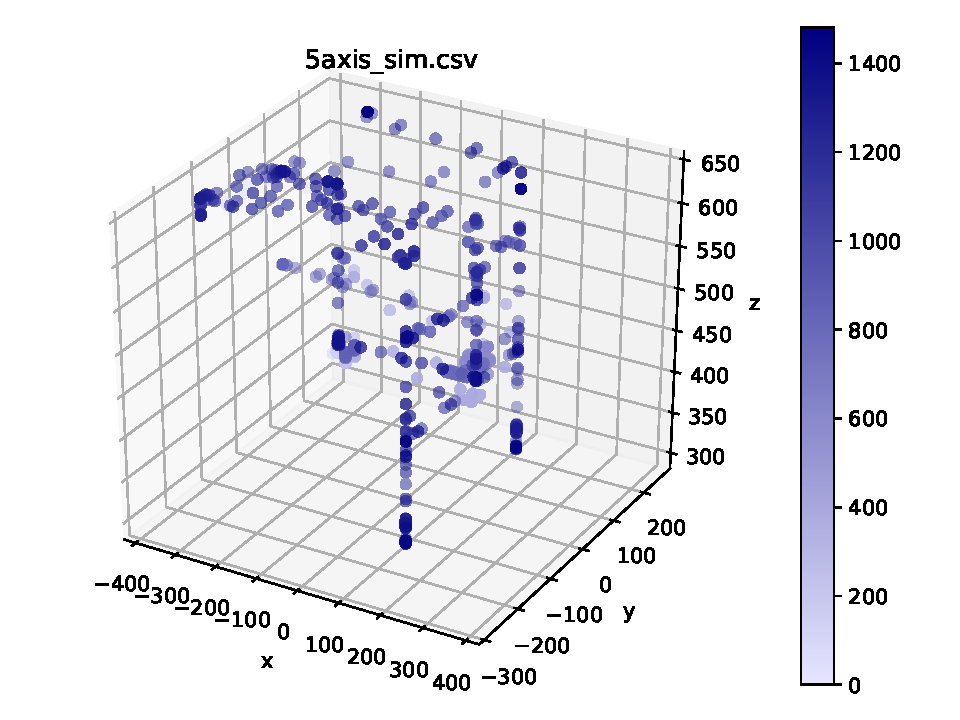
\includegraphics[width=\textwidth]{sim.pdf}
        \caption{Coordinates of simulated process}
    \end{subfigure}%
    ~
    \begin{subfigure}[t]{0.5\textwidth}
        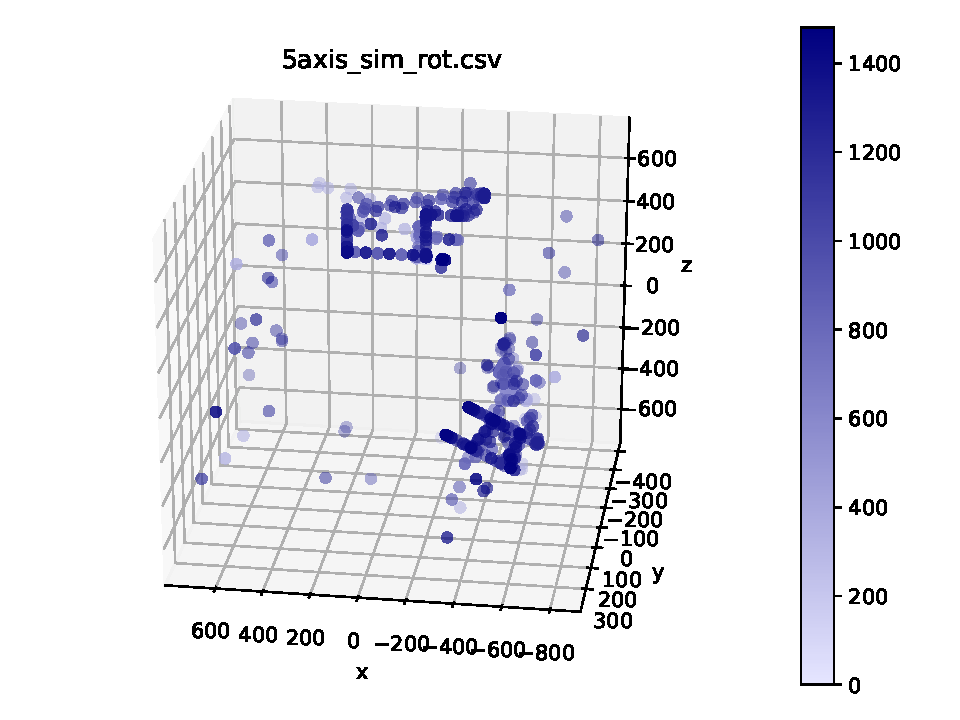
\includegraphics[width=\textwidth]{rot_sim.pdf}
        \caption{Attempted rotation}
    \end{subfigure}%

    \caption{Sad caption}
    \label{fig:rot}
\end{figure}

\end{document}
